\documentclass[10 pt]{beamer}

\usepackage{listings}
\usepackage{xcolor}
\usepackage{natbib,url}

\usepackage{color,fancybox,bm}
\usepackage{color}
\usepackage{booktabs}
\usepackage{threeparttable}
\usepackage{dashrule}
\usepackage{float}
\usepackage{graphicx}
\usepackage{amsmath}
\usepackage{fixltx2e}
\usepackage{amssymb}
\usepackage{rotating}
\usepackage{beamerthemeshadow}
\usepackage{graphicx}
\usepackage{subfigure}
\newtheorem{acknowledgement}[theorem]{Acknowledgement}
\newtheorem{algorithm}[theorem]{Algorithm}
\newtheorem{assumption}{Assumption}
\newtheorem{assumption1}{Assumption 1}
\newtheorem{assumptions}{Assumptions}
\newtheorem{axiom}[theorem]{Axiom}
\newtheorem{case}[theorem]{Case}
\newtheorem{thm1}[theorem]{Theorem 1}
\newtheorem{thm2}[theorem]{Theorem 2}
\newtheorem{claim}[theorem]{Claim}
\newtheorem{conclusion}[theorem]{Conclusion}
\newtheorem{condition}[theorem]{Condition}
\newtheorem{conjecture}[theorem]{Conjecture}
\newtheorem{criterion}[theorem]{Criterion}
\newtheorem{exercise}[theorem]{Exercise}
\newtheorem{notation}[theorem]{Notation}
\newtheorem{proposition}[theorem]{Proposition}
\newtheorem*{remark}{Remark}
\newtheorem{summary}[theorem]{Summary}
\newcommand{\nc}{\newcommand}
\nc{\tr}{\text{tr}}

\useoutertheme{infolines}
\setbeamercolor*{palette
primary}{use=structure,fg=structure.fg,bg=structure.fg!40!white}
\setbeamercolor*{palette
secondary}{use=structure,fg=white,bg=structure.fg!60!white}
\setbeamercolor*{palette
tertiary}{use=structure,fg=white,bg=structure.fg!90!white}
\setbeamercolor*{palette quaternary}{fg=white,bg=black}

\setbeamercolor*{sidebar}{use=structure,bg=structure.fg}

\setbeamercolor*{palette sidebar
primary}{use=structure,fg=structure.fg!10} \setbeamercolor*{palette
sidebar secondary}{fg=white} \setbeamercolor*{palette sidebar
tertiary}{use=structure,fg=structure.fg!50} \setbeamercolor*{palette
sidebar quaternary}{fg=white}

\setbeamercolor*{titlelike}{use=structure,fg=structure.fg,bg=structure.fg!20!white}

\setbeamercolor*{separation line}{} \setbeamercolor*{fine separation
line}{}

\setbeamercolor*{block title example}{fg=black}

\usefonttheme[onlysmall]{structurebold}

\newcommand{\ft}{\frametitle}
\newcommand{\bb}{\begin{block}}
\newcommand{\eb}{\end{block}}
\newcommand{\bi}{\begin{itemize}}
\newcommand{\ei}{\end{itemize}}
\newcommand{\be}{\begin{enumerate}}
\newcommand{\ee}{\end{enumerate}}
\newcommand{\bab}{\begin{alertblock}}
\newcommand{\eab}{\end{alertblock}}
\newcommand{\beb}{\begin{exampleblock}}
\newcommand{\eeb}{\end{exampleblock}}
\newcommand{\bc}{\begin{columns}}
\newcommand{\ec}{\end{columns}}
\newcommand{\ii}{\item}
\newcommand{\convas}{\stackrel{a.s.}{\rightarrow}}
\newcommand{\convp}{\stackrel{p}{\rightarrow}}
\newcommand{\convd}{\stackrel{d}{\rightarrow}}
\newcommand{\ba}{\begin{array}}
\newcommand{\ea}{\end{array}}

\newcommand{\Trans}  {\mathrm{T}}
\newcommand{\Ex}  {\mathbb{E}}
\newcommand{\Px}  {\mathbb{P}}
\newcommand{\RedText} {\textcolor[rgb]{1,0,0}}

\setbeamertemplate{theorems}[numbered]
\newtheorem*{lemmaC4}{Lemma}

\title[]{The Cure Model for Teeth Data}


\author{Fengyu Zhang}
\institute[]{Institute of Statistics \& Big Data \\ Renmin University of China
	
}

\date{}

\begin{document}
	
	\begin{frame}
	\titlepage
\end{frame}



\begin{frame}{Data Overview}
The data is about a kind of dental disease. The dataset contains 65890 observations of 20 variables. Here is a overview of the dataset:
\begin{figure}
	\centering
	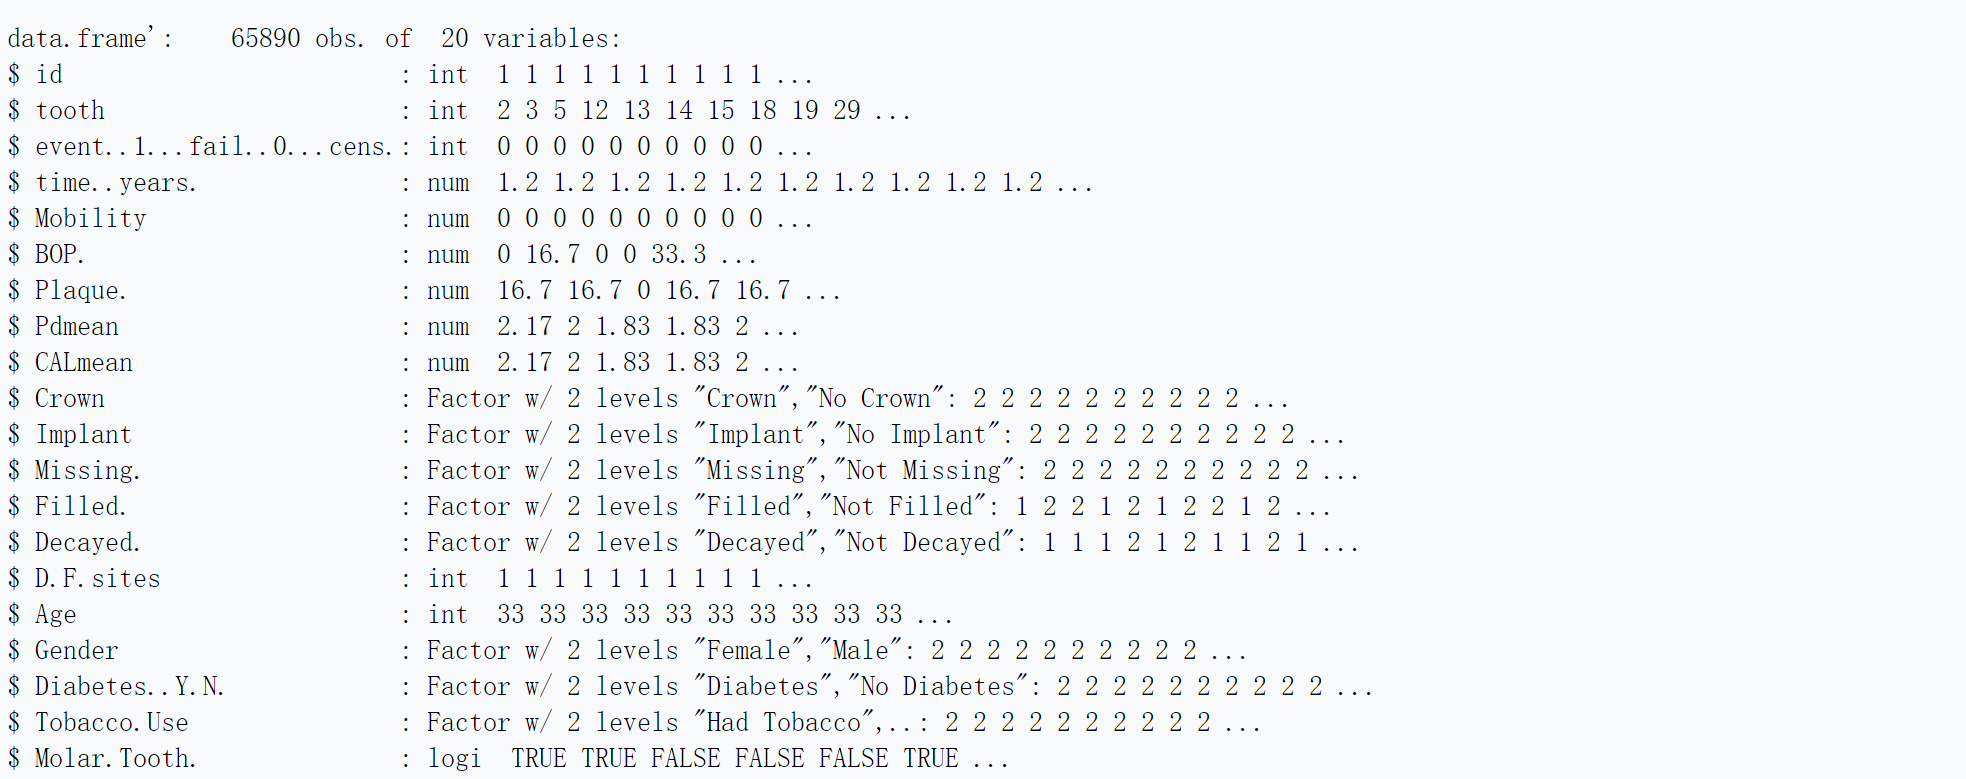
\includegraphics[width=1\textwidth]{figure/data_overview}
\end{figure}
Specific details are given in "Data\_Description.txt".
\end{frame}

\begin{frame}{Data Overview}
	In order to be operable, we select the observations with “tooth=2” which is a molar and rename some of the columns for convenience. Also, we remove some irrelevant variables. Here is the overview of the dataset that has been preprocessed:
	\begin{figure}
		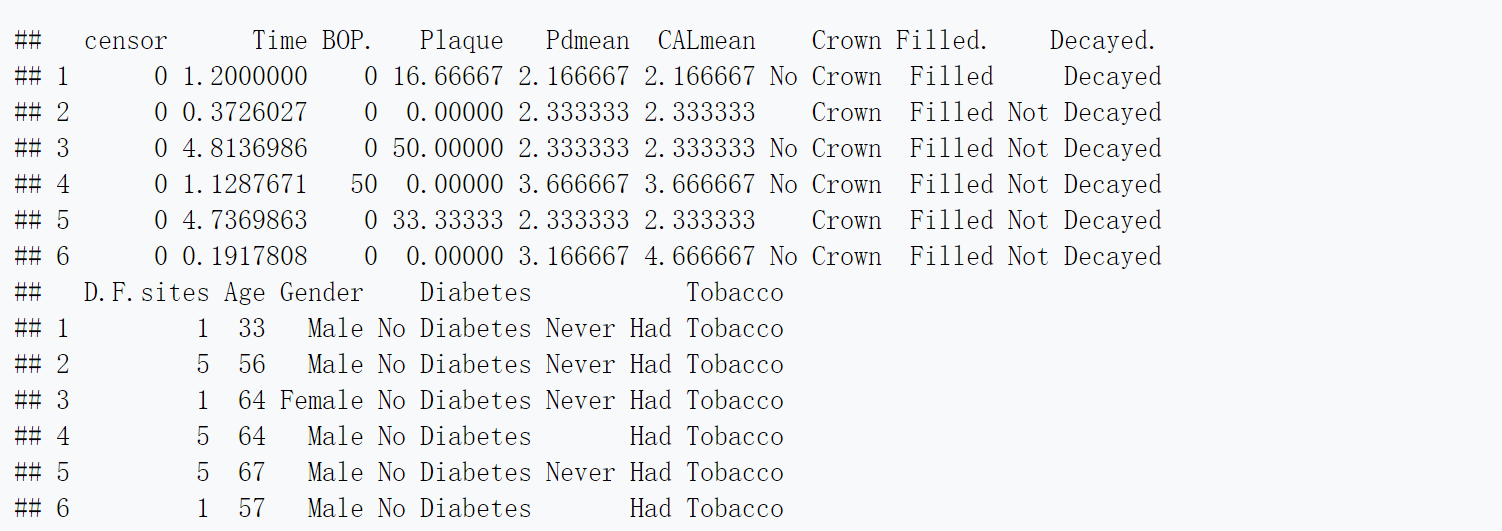
\includegraphics[width=1\textwidth]{figure/preprocess}
	\end{figure}
	*In practice, we need to transform the binary variables to 0-1 variables.
\end{frame}

\begin{frame}{Data Overview}
	A first look at the censor rate.
	\begin{figure}
		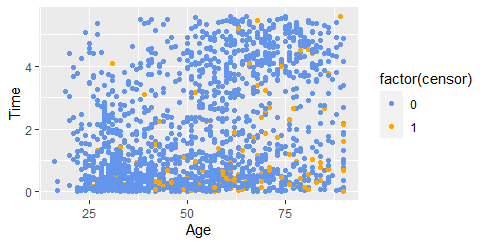
\includegraphics[width=1\textwidth]{figure/censor1}
	\end{figure}
Each point represents an observation and the 92\% of the observations are censored. We can see that the censor rate is high and a cure model seems therefore appropriate for these data.
\end{frame}

\begin{frame}{Cure model}
	\begin{itemize}
		\item 	In survival analysis, one usually assumes that all subjects under study will eventually experience the event of interest.
		\item   When the event of interest is the time until a patient progresses or relapses from a certain disease, then patients who are cured from the disease will never experience the event.
		\item 	Their survival time will be set to \textcolor[rgb]{1,0,0}{infinity}.
		\item   Cure models are survival models that have been developed to take this feature into account.
	\end{itemize}

\end{frame}

\begin{frame}{Cure model}
	\cite{Boag1949} and \cite{Farewell1982} originally proposed a mixture cure model which assumes that the survival function has the following form:
	\begin{equation}\label{equ:sur_fun}
		S(t|x,z) = P(T>t|x,z) = 1 - p(x) + p(x)S_u(t|z),\quad t\geqslant 0,
	\end{equation}
	where 
	\begin{itemize}
		\item 	$p(x)=\Px(B=1|X=x)$ is the conditional probability of being uncured (often referred to as the '\RedText{incidence}') with $B=I(T<\infty)$ the latent uncured status.
		\item $S_u(t|z)=\Px(T>t|B=1,Z=z)$ is the conditional survival function for the uncured subjects (often referred to as the '\RedText{latency}')
	\end{itemize}
	Here, the covariate vectors $X$ and $Z$ can contain (partially) the same covariates, but they can also be completely different.

\end{frame}

\begin{frame}{Cure model}
	For the part of latency ($S_u(t|z)$), we consider a Cox propotional hazards (PH) model (\citealt{Cox1972}) with the following form 
	\begin{equation}
	S_u(t|z) = S_0(t)^{\exp(\beta^\Trans z)}
	\end{equation}
	where $S_0(t)=\Px(T>t|B=1)$ is the baseline conditional survival function. The conditional hazard function is given by 
	$$\lambda_u(t|z)=\lambda_0(t)\exp(\beta^\Trans z),$$
	where $\lambda_0(t)$ is the baseline hazard function.
\end{frame}

\begin{frame}{Cure model}
	For the part of incidence (uncured rate $p(x)$), two models are considered. 
	\begin{enumerate}
		\item Logistic model (common assumption): $$p(x)=\frac{\exp(\gamma_0+\gamma^\Trans x)}{1+\exp(\gamma_0+\gamma^\Trans x)}$$
		for some parameter vector $\gamma$ and an intercept $\gamma_0$. The logistic model is easy to interpret and estimate                                                                                                                                                                                                                                                                                                                                                                                                                                                        
		\item Single-index model:
		$$p(x) = g(\gamma^\Trans x)$$
		for any smooth link function $g$ with values between 0 and 1. The single-index model has nonparametric link function and therefore much more flexibel than the logistic model. Besides, it does not suffer from the curse-of-dimensionality problems.
	\end{enumerate}
\end{frame}

\begin{frame}{Estimation}
		In survival analysis, we usually observe the couple $(Y,\delta)$ instead of the survival time $T$, where $Y=\min (T,C), \delta = I(T\leqslant C)$, and $C$ is the censoring time. As often, we assume $T$ and $C$ are independent given the covariates $X,Z$. 
		
		Denote $(Y_i,\delta_i,X_i,Z_i),i=1,\ldots,n$ be i.i.d. realizations of $(Y,\delta,X,Z)$, the likelihood function takes the form
		\begin{equation}\label{equ:L_c}
			L = \prod_{i=1}^{n}\{p(X_i)f_u(Y_i|Z_i)\}^{\delta_i}\cdot \left[\{1-p(X_i)\}+p(X_i)S_u(Y_i|Z_i)\right]^{1-\delta_i}.
		\end{equation}
		where $f_u(t|z) = -(d/dt)S_u(t|z)$ is the conditional density function. The likelihood has two types of contributions: from censored and from the uncensored observations. 
\end{frame}

\begin{frame}{Estimation}
	We use EM algorithm to handle the fact that the cure status $B_i$ is unobserved. The complete-data likelihood is given by
	\begin{equation}\label{equ:com_data}
	\begin{aligned}
		L_c =& \prod_{i=1}^{n}\{p(X_i)\lambda_u(Y_i|Z_i)S_u(Y_i|Z_i)\}^{B_i \delta_i}\times \\ &\left[\{1-p(X_i)\}^{1-B_i}+\{p(X_i)S_u(Y_i|Z_i)\}^{B_i} \right]^{1-\delta_i}
	\end{aligned}
	\end{equation}
	Then we need to calculate the conditional expectation of the log-likelihood given the observed data and the current parameter values. As the log-likelihood is linear in $B$, it is the same as computing $$\Ex(B_i|\mathcal{O},\Theta^{(m-1)}) := W_i^{(m)},$$
	where $\mathcal{O} = \{(Y_i,\delta_i,X_i,Z_i),i=1,\ldots,n\}$ are observed data and $ \Theta = (\gamma,\beta,S_0)$ for logistic model and $\Theta = (\gamma,\beta,S_0,g)$ for single-index model.
\end{frame}

\begin{frame}{Estimation}
	In M-step, we maximize the expected log-likelihood which is obtained by replacing $B_i$ by $W_i^{(m)}$ in the equation (\ref{equ:com_data}):
	\begin{equation}
	\begin{aligned}
	\tilde{L}_c=& \prod_{i=1}^{n}\{p(X_i)\lambda_u(Y_i|Z_i)S_u(Y_i|Z_i)\}^{W_i^{(m)} \delta_i}\times \\ 
		&\left[\{1-p(X_i)\}^{1-W_i^{(m)}}+\{p(X_i)S_u(Y_i|Z_i)\}^{W_i^{(m)}} \right]^{1-\delta_i}.
	\end{aligned}
	\end{equation}
	After some algebra, $\tilde{L}_c$ can be written as the product of two parts:
	\begin{equation}
	\begin{aligned}
	\tilde{L}_c &= \prod_{i=1}^n \left[p(X_i)^{W_i^{(m)}}\{1-p(X_i)\}^{1-W_i^{(m)}}\right]\times 
	\prod_{i=1}^n \{\lambda_u(Y_i|Z_i)^{\delta_i}S_u(Y_i|Z_i)\}^{W_i^{(m)}} \\
	&= \tilde{L}_1 \times \tilde{L}_2.
	\end{aligned}
	\end{equation}
	It can be maximized separately for the two parts of the model.
\end{frame}

\begin{frame}{Estimation}
	Although the framework of the EM algotirhm is constructed, one problem is that how to estimate the parameters when we use the single-index model in the incidence part. \cite{Ich1993} proposed a leave-one-out kernel estimator of $g(\gamma^\Trans X_i)$:
	$$\sum_{j \neq i}^{n} \frac{K\left(\frac{\gamma^{t} X_{i}-\gamma^{t} X_{j}}{h}\right)}{\sum_{l \neq i}^{n} K\left(\frac{\gamma^{t} X_{i}-\gamma^{t} X_{l}}{h}\right)} B_{j}.$$
	We need to replace $B_j$ by $W_j^{(m)}$ obtained in the E-step and then the estimator becomes
	\begin{equation}\label{equ:ker_est}
		\tilde{g}_{-i}^{(m)}\left(\gamma^{t} {X}_{i}\right)=\sum_{j \neq i}^{n} \frac{K\left(\frac{\gamma^{t} X_{i}-\gamma^{t} X_{j}}{h}\right)}{\sum_{l \neq i}^{n} K\left(\frac{\gamma^{t} X_{i}-\gamma^{t} X_{l}}{h}\right)} W_{j}^{(m)}
	\end{equation}
	The kernel estimator (\ref{equ:ker_est}) is substitued in $\tilde{L}_1$, and $\gamma$ is estimated by maximizing the likelihood.
\end{frame}

\begin{frame}{Estimation}
	Another problem is that how to estimate the latency ($\tilde{L}_2$). Note that 
	$\tilde{L}_2=\prod_{i=1}^{n}\left[\left\{\lambda_{0}\left(Y_{i}\right) \exp \left(\boldsymbol{\beta}^{t} \boldsymbol{Z}_{i}\right)\right\}^{\delta_{i}} \exp \left\{-\Lambda_{0}\left(Y_{i}\right) \exp \left(\boldsymbol{\beta}^{t} \boldsymbol{Z}_{i}\right)\right\}\right]^{W_{i}^{(m)}}.$\\
	\cite{Sy2000} propose a profile likelihood approach to estimate $\beta$.\\
	First, given a fixed $\beta$, $\Lambda_{0}$ is estimated nonparametrically by 
	\begin{equation}\label{equ:Lambda}
		\sum_{j: Y_{(j)} \leq t} \frac{D_{j}}{\sum_{k \in R_{j}} W_{k}^{(m)} \exp \left(\boldsymbol{\beta}^{t} {Z}_{k}\right)},
	\end{equation}
	where $Y_{(j)}$ are order statitics, $D_j$ is the number of events at time $Y_{(j)}$ and $R_j$ is the risk set before $Y_{(j)}$.
	Second, we plug (\ref{equ:Lambda}) in $\tilde{L}_2$, obtaining the partial likelihood
	\begin{equation}\label{equ:L2}
		\breve{\mathrm{L}}_{2}=\prod_{i=1}^{n}\left\{\frac{\exp \left({\beta}^{t} {Z}_{i}\right)}{\sum_{k \in R_{i}} W_{k}^{(m)} \exp \left({\beta}^{t} {Z}_{k}\right)}\right\}^{\Delta_{i}}
	\end{equation}
	The MLE of $\beta$ denoted by $\hat{\beta}^{(m)}$ is obtained by maximizing (\ref{equ:L2}). Then we plug $\hat{\beta}^{(m)}$ in (\ref{equ:Lambda}) to obtain $\hat{\Lambda}_0^{(m)}(t)$. We do alternative iterations until convergence.
\end{frame}

\begin{frame}{Data Application}
\begin{table}[htbp]
	\centering
	\caption{Parameter Estimations, Std.error and Wald's test}
	\small
	\begin{tabular}{lrrrrrr}
		\hline
		& \multicolumn{3}{c}{SIC cure model} & \multicolumn{3}{c}{LC cure model} \\
		\hline
		Incidence & \multicolumn{1}{l}{Estimate} & \multicolumn{1}{l}{Std.error} & \multicolumn{1}{l}{p-value} & \multicolumn{1}{l}{Estimate} & \multicolumn{1}{l}{Std.error} & \multicolumn{1}{l}{p-value} \\
		\hline
		(intercept) & \multicolumn{1}{c}{-} & \multicolumn{1}{c}{-} & \multicolumn{1}{c}{-} & -4.54406 & 1.573907 & 0.003888 \\
		Age     & 0.56649 & 0.180257 & \RedText{0.0016741} & 0.031461 & 0.016599 & \RedText{0.058042} \\
		Gender  & -0.05871 & 0.346062 & 0.8652774 & -0.01342 & 0.55367 & 0.980664 \\
		BOP     & 0.6242  & 0.294932 & \RedText{0.0343093} & 1.692404 & 0.834437 & \RedText{0.04254} \\
		Plaque  & -0.4325 & 0.269344 & 0.1083279 & -0.00462 & 0.815525 & 0.995481 \\
		Pdmean  & -0.08126 & 0.244503 & 0.7396307 & 0.152681 & 0.281289 & 0.587275 \\
		CALmean & 0.303903 & 0.198951 & 0.12663 & 0.201554 & 0.165835 & 0.224218 \\
		&         &         &         &         &         &  \\
		\hline
		latency & \multicolumn{1}{l}{Estimate} & \multicolumn{1}{l}{Std.error} &
		 \multicolumn{1}{l}{p-value} & \multicolumn{1}{l}{Estimate} & \multicolumn{1}{l}{Std.error} & \multicolumn{1}{l}{p-value} \\
		 \hline
		Age     & -0.02421 & 0.010842 & \RedText{0.0255254} & -0.02177 & 0.016181 & 0.178525 \\
		Gender  & 0.148134 & 0.220341 & 0.5013959 & 0.193319 & 0.572714 & 0.735703 \\
		BOP     & 0.815028 & 0.426396 & 0.055949 & -0.29098 & 0.593112 & 0.623712 \\
		Plaque  & -0.77723 & 0.392359 & 0.0476001 & -0.68691 & 0.794442 & 0.387237 \\
		Pdmean  & 0.258177 & 0.160801 & 0.1083693 & -0.02163 & 0.224441 & 0.923235 \\
		CALmean & 0.343105 & 0.119735 & \RedText{0.0041631} & 0.359877 & 0.162896 & \RedText{0.027157} \\
		\hline
	\end{tabular}%
	\label{tab:addlabel}%
\end{table}%
\end{frame}

\begin{frame}{Data Application}
	
	\begin{itemize}
		\item According to the table, for the latency part, the effects for age, gender, Plaque and CALmean have the same direction and the estimates are very close. Only CALmean affects significantly the survivial time of uncured subjects in both of the two models.
		\item For the incidence part, we compare the predicted error of the incidence. First we divided the dataset into a training and test subsut, following 2/3-1/3 recommendations of \cite{Hastie2009}. We use the training set to estimate the parameters and calculate the prediction error which is given by
		\begin{equation}\label{equ:PE}
			PE =-\sum_{j=1}^{n_{test}} \log \left[\hat{p}\left({x}_{j}^{\text {test}}\right)^{\hat{w}_{j}}\left\{1-\hat{p}\left({x}_{j}^{\text {test}}\right)\right\}^{1-\hat{w}_{j}}\right]
		\end{equation}
		After computing, the prediction error for the SIC model equals to 57.65, while it is equal to 70.93 for the LC model, which means that the SIC model performs better in predicting the uncured status.
	\end{itemize}
\end{frame}

\begin{frame}{Reference}
	\bibliographystyle{jasa}
	\bibliography{Ref.bib}
\end{frame}

\end{document}

